\chapter{Networks}

In this chapter, we'll learn about how the Internet and different kinds of networks work. The Internet is a giant network composed of many different smaller networks. Each of these networks have to link together various devices to allow devices within a network to communicate with each other and allow devices within one network to communicate with another network. There are complex protocols that dictate how different kinds of devices should communicate with each other, but you don’t have to understand the details of these protocols to understand how devices can communicate with each other.

In addition to being interesting and important to understanding technology, understanding networks is very practical. Many companies look for Internet Technology or IT specialist that understand how networks work. Taking a test like the Network+ certification or A+ certification allows access to these jobs. These tests are knowledge based, so you don’t need practical experience to do well on them. They qualify you for entry level positions that pay around \$50,000 a year. If you’re interested in preparing for these exams, there are many books that can help you prepare. For instance, ``CompTIA A+ Certification All-in-One Exam Guide, Ninth Edition (Exams 220-901 \& 220-902).''

In this section we'll start by examining how a device could communicate with another device in a small network and build up to understanding how a device can communicate to a device across the world.

\section{Local Area Networks}

A local area network (LAN) is a relatively small network that is often used in homes, schools, individual office buildings, or another small building. In a local area network each computer connected to the network will be assigned an Internet Protocol Address (IP address) for use within the network. If computer A wants to send a message to computer B within the same address, computer A would refer to computer B by its IP address. IP addresses are 32 bit numbers that are written with dots between each byte. For instance, the address 192.168.0.1 usually refers to the machine that enters the address, a location known as ``local host.''

If computer B wants to receive messages from computer A, it could want to receive messages for multiple reasons. To allow this, messages sent to another computer have to include what “port” they want to use. A port is a number used to identify a particular reason that another machine could want to receive a message. Many ports, especially ports with smaller numbers, have conventional services that they correspond to. For instance, port 80 corresponds to a web server, port 443 corresponds to a web server using encryption, and port 5432 corresponds to a particular kind of database.

\begin{figure}
	\centering
	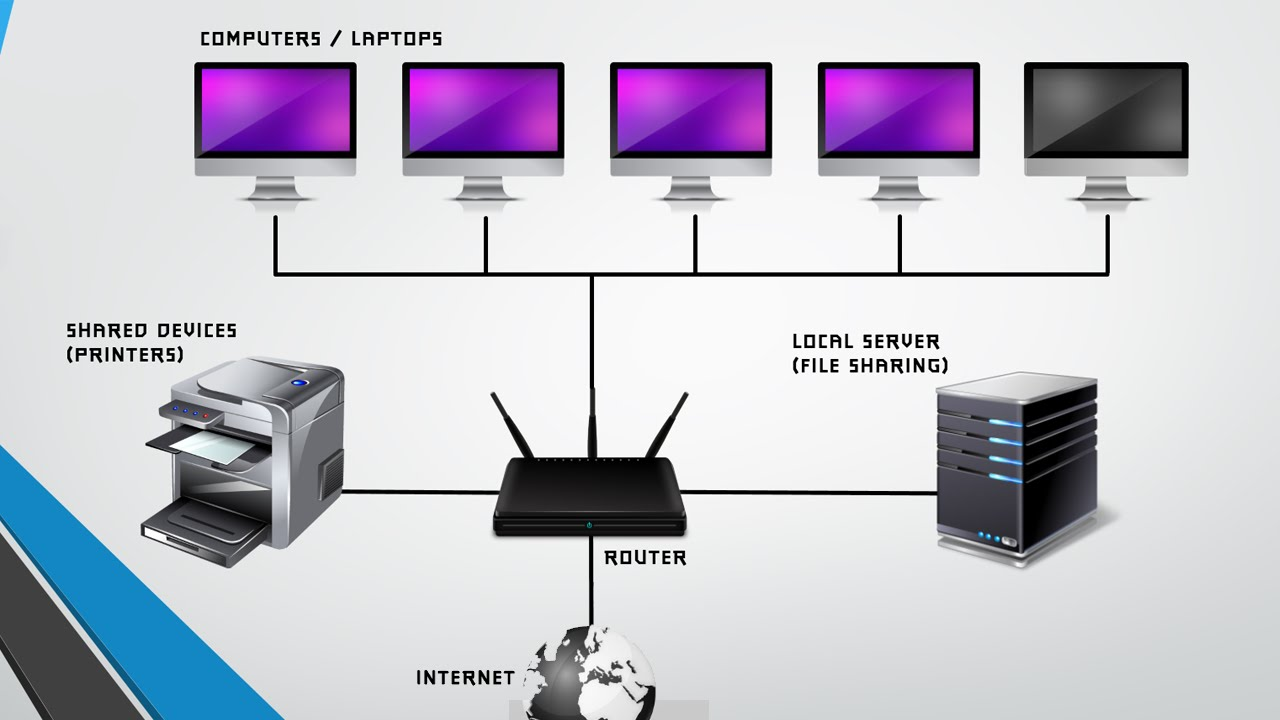
\includegraphics[width=0.85\textwidth]{images/lanExample.png}
	\caption{Local Area Network Example}
	\label{fig:windows:file}
\end{figure}

The simplest way for multiple computers to communicate is to be connected together by a cable. If two machines want to talk with each other and the computers are connected to each other by a cable, a machine would broadcast the message to all other machines along with the address the machine was intended for. The machine the message was intended for would pick up the message and all others would hopefully discard it, although they could still see the contents if they wanted to.

\begin{figure}
	\centering
	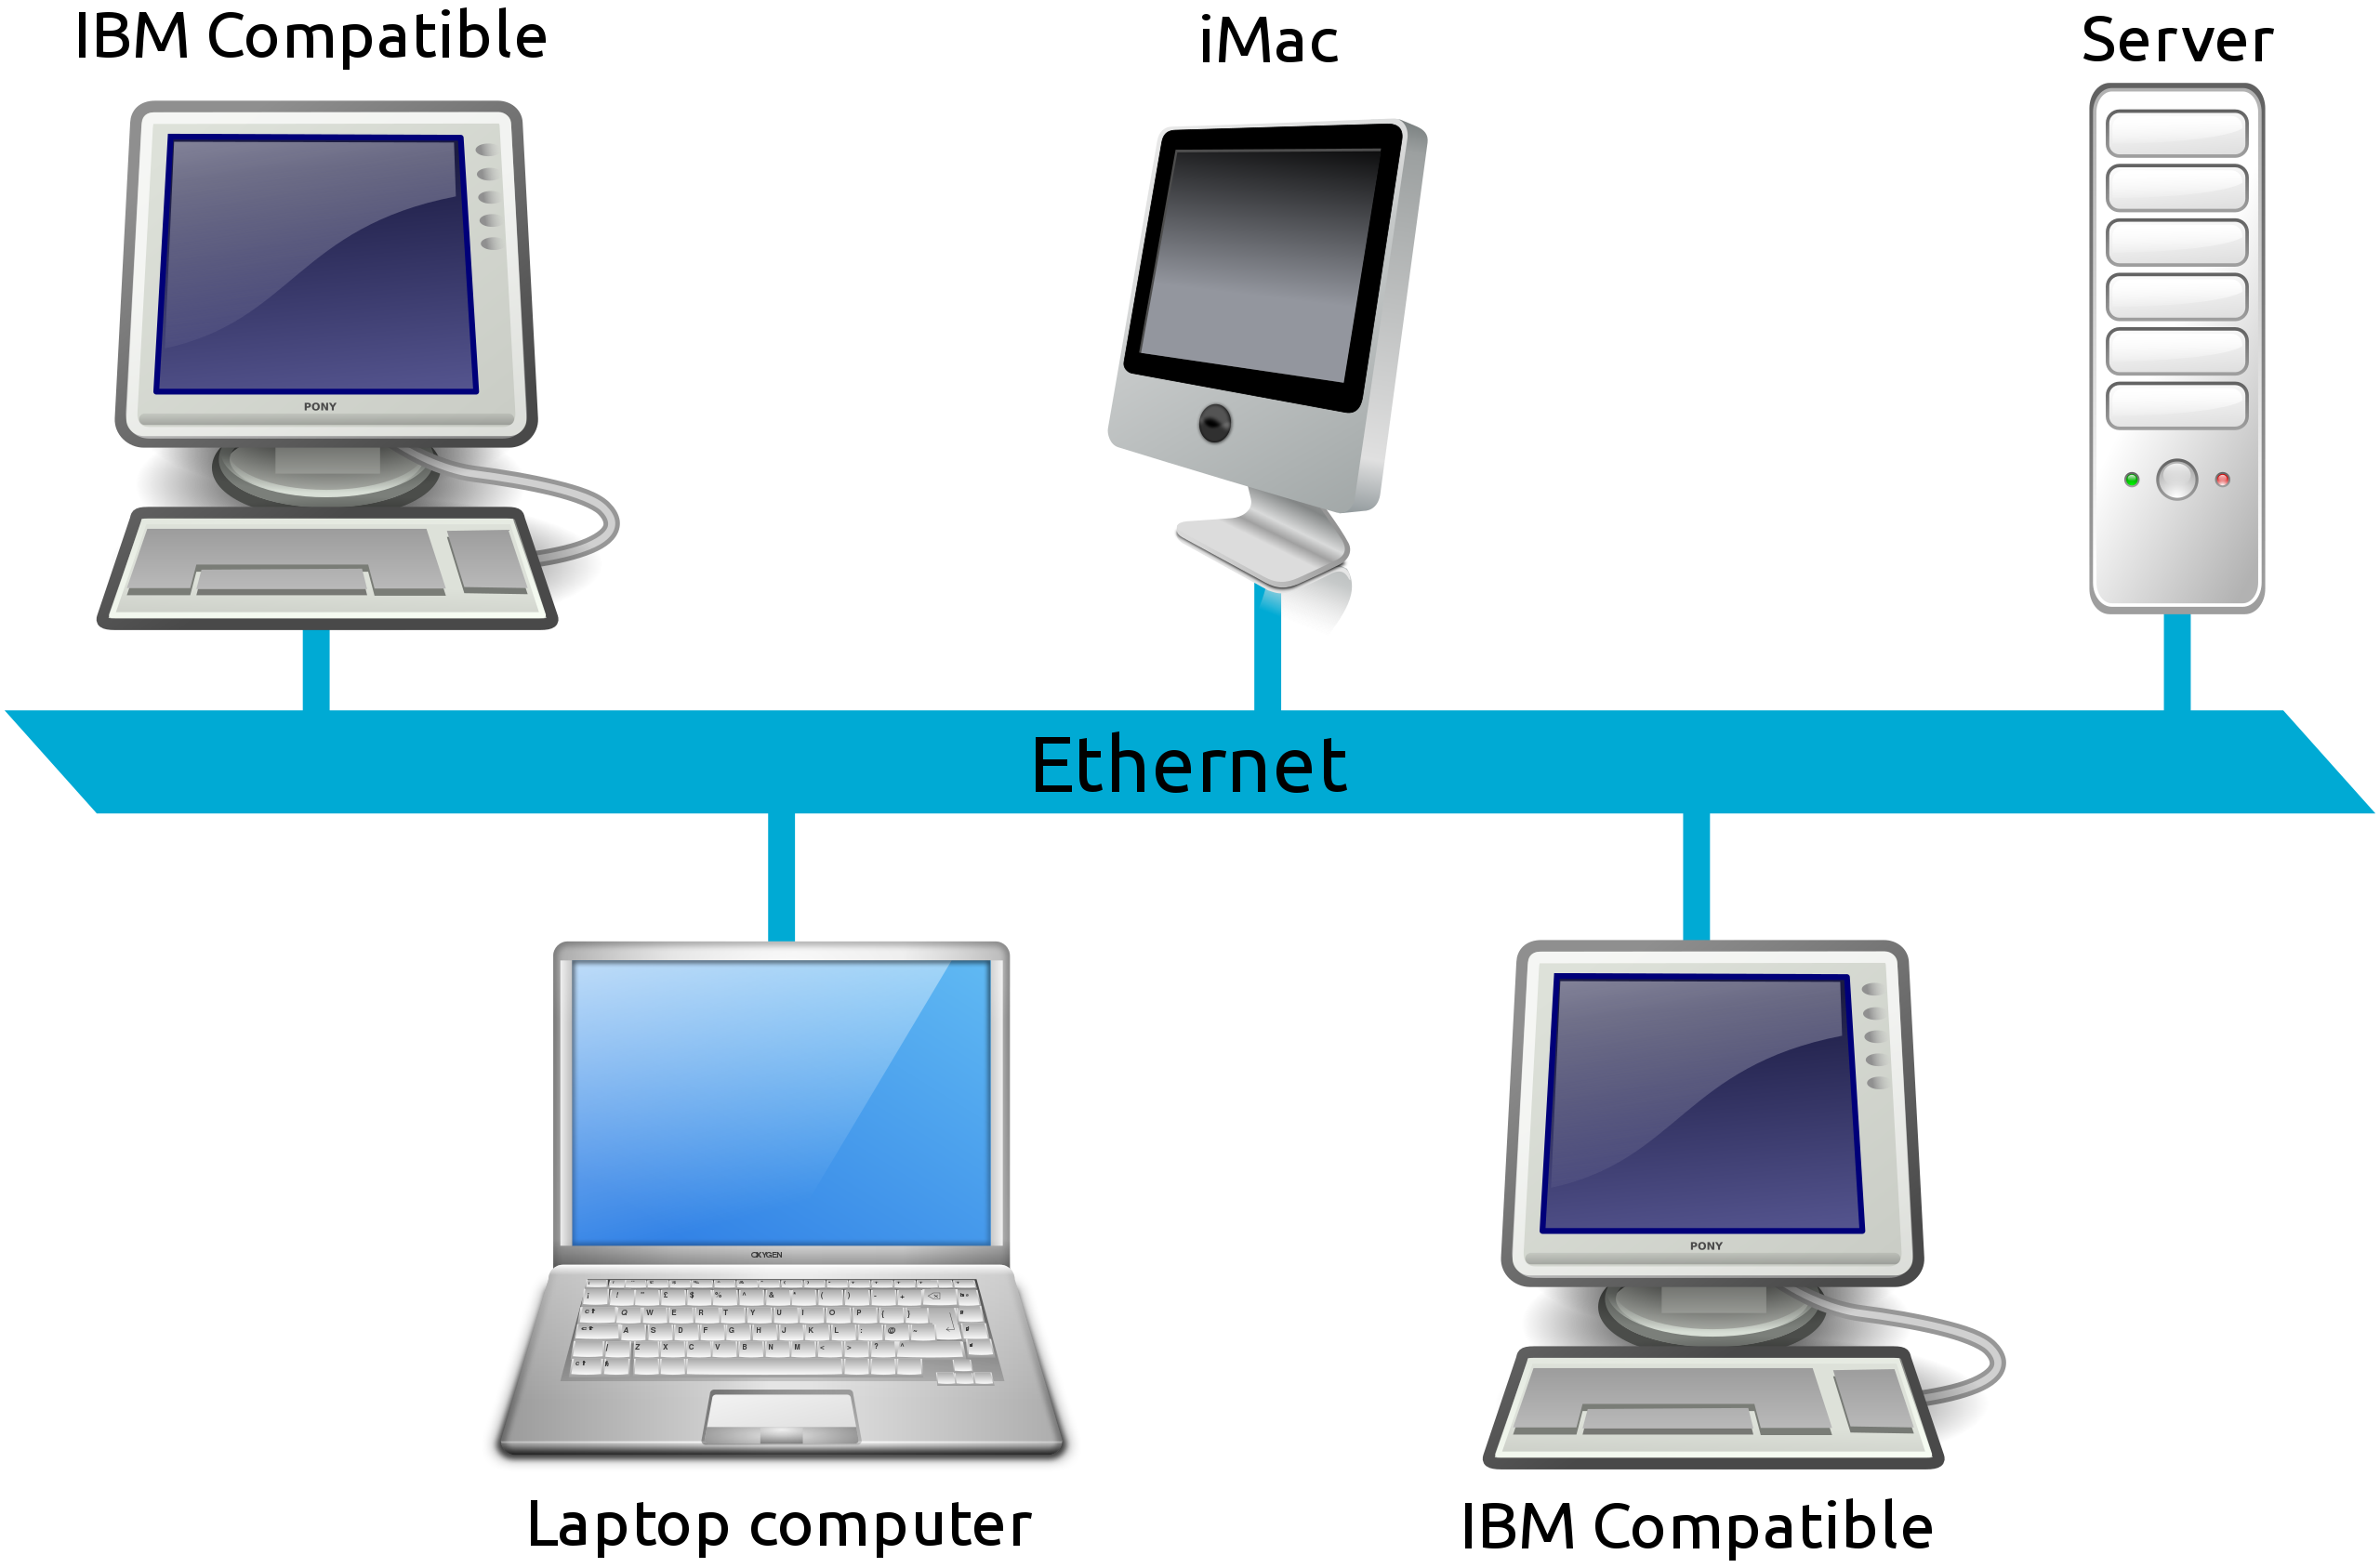
\includegraphics[width=0.85\textwidth]{images/ethernetExample.png}
	\caption{Example of communicating over Ethernet}
	\label{fig:windows:file}
\end{figure}

A switch is a more sophisticated way to route information between computers on the same network than an Ethernet cable. A switch knows how to allow machines on the same network to communicate. In larger local area networks many different switches could be used to carry messages between different sets of computers. In the case of wireless devices, the wireless’s devices signals are collected by an access point and then translated to signals that can be sent across a physical wire to switches.

\begin{figure}
	\centering
	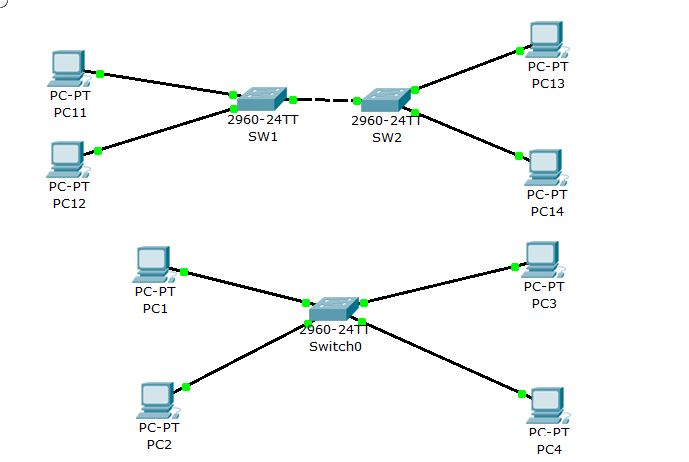
\includegraphics[width=0.85\textwidth]{images/switchExample.png}
	\caption{Example of communicating over Ethernet}
	\label{fig:windows:file}
\end{figure}

If devices within the local area network want to communicate with devices outside the local area network, they’ll need to go through a router. A router is the machine that assigns IP addresses to other machines in the same local area network. While these machines can use the IP addresses to communicate with other machine within the same local area network, they can’t use the IP address to communicate directly with machines outside the local area network. The router has an IP address that it uses to communicate with other devices outside of the LAN. If a device within the LAN wants to communicate with a device outside of the LAN, the router makes the request for the device inside the LAN and changes the IP address to the IP address of the router. It maintains state about the device that sent the request to the router so that when the target of the request replies, the router can forward the reply to the right device in the network.


Consider the example given in figure 7.4. If the machine with the IP address 192.168.100.3 wants to send a request to a machine with the IP address 209.131.36.158 using port 80, it will forward that request to the router. The router will then send change the requesting IP address to its IP address of 145.12.131.7 and when it receives the reply from 209.131.36.158, it will forward that reply to 192.168.100.3.

\begin{figure}
	\centering
	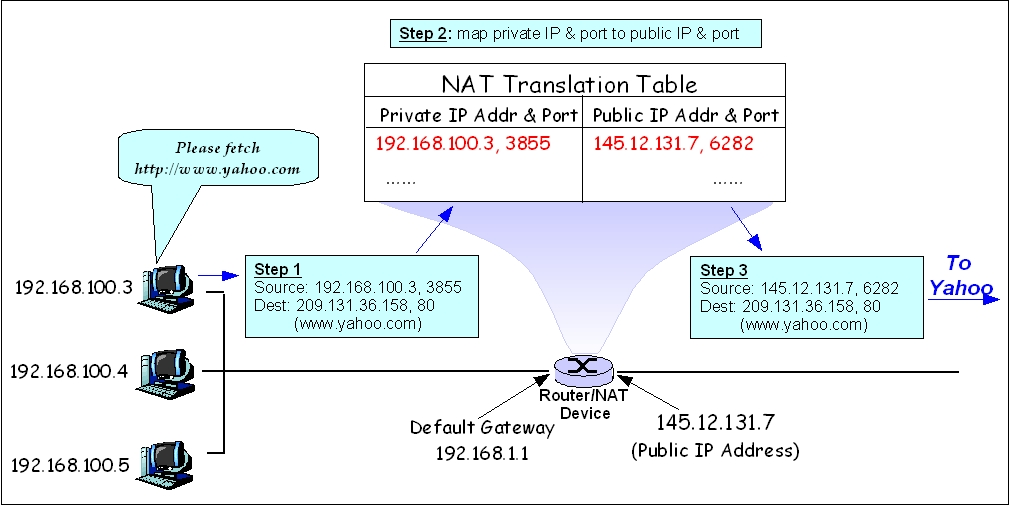
\includegraphics[width=0.85\textwidth]{images/routingExample.png}
	\caption{Network routing}
	\label{fig:windows:file}
\end{figure}


One of the primary reasons this process occurs is because there are only $2^{32}$ possible IP addresses in the most used version of the IP protocol (the number of numbers that can be created using 32 bits). This may seem like a lot, but $2^{32}$ is about 4.3 billion, and there are many more devices that can be connected to the Internet than this! This scheme allows many of the device addresses to be reused.

\section{Wide area networks}

Wide area networks refer to large networks that usually combine multiple local area network. The definition of what is considered a wide area network varies, but it usually involves connecting local area networks that are miles apart. In this section we’ll look at an outline of how large networks are connected to give an intuition for how devices in the modern world communicate.

Almost all information between computers will travel through wires for a significant portion of the time, with the major exception being information that is beamed up to a satellite and then beamed down to another device. For two local area networks to communicate over large distances, they usually enlist the service of an Internet Service Provider (ISP). An ISP like Time Warner Cable or Comcast is responsible for ensuring that there is a path between two separate local area networks that want to contribute. When connecting to an ISP, the LAN would have a wire that connects the LAN to the network of wires the ISP uses to route information between different LANs.

The ISP would make agreements with different autonomous systems (ASs) to be able to route traffic through the autonomous system so that it doesn’t have to own the cable used to route data between different places. These ASs advertise what other ASs they can communicate with using the Boarder Gateway Protocol. The protocol can allow ASs to figure out if there’s a path to another AS through an AS they’re directly connected to.

To send information across the world, there are cables running through the ocean operated by Internet Service Providers. There are cables acros mountains, deserts, and other challenging terrains to enable the flow of information.

\referencessection

Muhammadlilg. (2014, October 21). Retrieved June 16, 2019.\\

Otome, S. O. (n.d.). What are the reasons for not putting multiple subnets on the same VLAN?
